% Schnelles Übersetzen scheitert wegen µm in Titel Bach.2012!!
\documentclass[12pt,a4paper,onecolumn]{scrartcl}
\usepackage[utf8]{inputenc}
\usepackage{adjustbox}
\usepackage{amsfonts}
\usepackage{amsmath}
\usepackage{amssymb}
\usepackage{array}
\usepackage[ngerman]{babel}
\usepackage[backend=biber,natbib=true,hyperref=true,
			style=draft,maxnames=2,maxbibnames=2, isbn=false]{biblatex} % STYLE draft SPÄTER NOCH GEGEN authoryear TAUSCHEN!!!!!!
\usepackage{caption, booktabs}
\usepackage{chngcntr} % Damit Zählungen von Abb und Co innerhalb sections mögl
\usepackage{csquotes}
\usepackage{float}
\usepackage[left=2.5cm,right=2.5cm,top=2.5cm,bottom=2.5cm,head=14.5pt]{geometry}
\usepackage[toc,acronym,nonumberlist,translate=babel]{glossaries}
\usepackage{graphicx}
\usepackage{grffile} % to allow underscores in filenames (pics&co)
\usepackage{hyperref}
\usepackage{lmodern}
\usepackage{makecell}
\usepackage{mathtools}
\usepackage{paralist}
\usepackage{pdfpages}
\usepackage[section]{placeins} % to keep figures in section
\usepackage{scrlayer-scrpage} % Zur Anpassung der Kopf- und Fußzeilen
\usepackage{subfig}
\usepackage{tabularx}
%\usepackage[scaled]{uarial} % Schriftart
\usepackage{underscore}
\usepackage{url}
\usepackage{wrapfig}

\addbibresource{literatur.bib} %% Einbinden der bib-Datei
\DefineBibliographyStrings{ngerman}{
	andothers = {{et\,al\adddot}},}

\def\theequation{\thesection.\arabic{equation}} % Formeln beginnen mit Abschnittssnummer
\linespread{1.0} % Zeilenabstand
\pagestyle{scrheadings}
\clearpairofpagestyles % Löschen der Platzhalter
\counterwithin{figure}{section} % damit figure je section neu gezählt werden

\newcommand*\mytitle{Bachelorthesis: Aussortierte Elemente}
\newcommand*\mysubtitle{Bachelorarbeit}
\newcommand*\myauthor{Marco Schulz}
\newcommand*\mydate{05.05.2021}
\newcommand{\cotwo}{CO\textsubscript{2}}

\begin{document}
\begin{titlepage}
\begin{center}
{\LARGE \textsc{\mysubtitle}} \bigskip \\
{\huge \textsf{\mytitle}} \bigskip \\
{\Large \myauthor \ - Matrikelnummer 7345692} \smallskip \\
{\Large Fassung vom \mydate} \bigskip \\
\begin{figure}[H]
\centering

\includegraphics[width=60mm]{bilder/unilogo.png}
\end{figure}
\bigskip
{\Large Institut für Geophysik und Meteorologie}
\bigskip
{\Large \\ Universität zu Köln}
\vspace{4cm}
\\
\end{center}
\begin{tabbing}
Erstgutachter: \quad  \= Prof. Yaping Shao (yshao@meteo.uni-koeln.de) \\[2ex]
Zweitgutachter:  \>  Dr. Hendrik Elbern (he@eurad.uni-koeln.de)
\end{tabbing}
\end{titlepage}
\setcounter{page}{2}
\ofoot{\pagemark}
\chead{{\small \mytitle}}
\automark{section}
\tableofcontents
\newpage

\subsection{Der südliche Ozean}

Schätzungsweise 45-62 \% der gesamten Wärmezunahme zwischen 2005 und 2017 in den oberen 2000m des globalen Ozeans entfielen auf den südlichen Ozean \citep{IPCCpol.2019}. Auch im tiefen Ozean $>2000m$ fand wahrscheinlich eine Erwärmung statt. Zusammen mit dem steigenden Eintrag von Süßwasser durch abschmelzende Eisschilde führt diese Erwärmung zu  einer zunehmenden Stratifizierung der oberen Ozeanschichten. Durch diese höhere hydrodynamische Stabilität wird  der Austausch von Nährstoffen in lichtdurchflutete Schichten erschwert, sodass die dortige Produktion von Phytoplankton beeinträchtigt ist. In der Arktis führten die Veränderungen in der Eisbedeckung zu einer erhöhten Nettoprimärproduktion, Phytoplankton-Blüten treten früher im Jahr auf. Rund um die Antarktis kann dies allerdings nicht pauschal beobachtet werden \citep{IPCCpol.2019}. Allerdings wird eine Südwärtsverlagerung des antarktischen Krillvorkommens vermutet. Derzeitige Klimaprognosen deuten daraufhin, dass die Nettoprimärproduktion in Arktis und Antarktis erhöhen , aber gleichzeitig in tropischen Gewässer deutlich sinken wird. Grundsätzlich bietet der südliche bzw. antarktische Ozean ein hohes Potential für die Produktion von Phytoplankton. Im (südhemisphärischen) Sommer sind große Teile der oberen Ozeanschichten ausreichend lichtdurchflutet und Nährstoffe (mit Ausnahme von löslichem Eisen) können durch das allgemeine Aufströmen aus der Tiefe an die Oberfläche transportiert werden \citep{Martin.1990}. -  Der antarkische Zirkumpolarstrom kann je nach Zone verschiedene chemikalische Eigenschaften aufweisen:

\begin{enumerate}
\item Subtropische Front
\item Subantarktische Zone
\item Subantarktische Front
\item polare Frontzone
\item Polarfront
\item Antarktische Zone
\item südliche Front des antarktischen Zirkumpolarstroms
\item südliche Grenze des antarktischen Zirkumpolarstroms
\end{enumerate}

\section{Anpassungen nach der ersten Simulation}
Die Ergebnisse der WRF-Simulation sollten in einem ersten Schritt durch eine grobe Übersicht auf Plausibilität, d.h. der wahrscheinlichen Abweichung von der Realität überprüft werden. Da ein relativ langer Zeitraum von 12 Tagen simuliert wird, sind auch größere Abweichungen wahrscheinlich. Ganz allgemein sind Wetterprognosen i.d.R. nur für die ersten Tage wirklich präzise. Die Wahrscheinlichkeit, dass das berechnete Wetter eintritt nimmt dann aufgrund des chaotischen Verhaltens der Atmosphäre und den beschränkt zur Verfügung stehenden diskreten Startwerten stark ab \textbf{(Quelle ergänzen)}. Beobachtungs- bzw. Reanalysedaten werden dem Modell zum Startzeitpunkt und an den Rändern geliefert. Die Zustände der zeitlich und räumlich dazwischen liegenden Gitterpunkte sind dann (ausschließlich) vom Modell simuliert (\textbf{Quelle Sven, nochmal checken}). Für den Großteil des untersuchten Gebietes liegen ohnehin keine Beobachtungsdaten vor. Der australische Kontinent ist relativ dünn mit Wetterstationen besetzt und Beobachtungen durch Satelliten sind hinsichtlich  zeitlicher und räumlicher Auflösung ebenfalls häufig relativ grob. Darüber hinaus können die interessanten Parameter meist nur indirekt ermittelt werden.\\

Dennoch können einfache Vergleiche einen ersten Eindruck von der Qualität der Simulation vermitteln. Hierzu wurden die simulierten Staubkonzentrationen und Emissionen mit Satellitenbildern, Beobachtungsdaten und Schätzungen aus der diesbezüglichen Literatur verglichen. Der Abgleich mit den (Echt-Farben-) Satellitenbildern zeigt, dass die Fortbewegung und Ausdehnung der Staubwolke vom Modell grundsätzlich erfasst wird. Auf Abbildung \ref{fig:wrf_sat} ist jedoch ebenfalls gut sichtbar, dass das Modell zu späteren Zeiten eine deutlich höhere Staubkonzentration im Nordwesten Australiens simuliert, als von den Satellitenbildern direkt ableitbar wäre. Dabei ist zu beachten, dass die (Echt-Farben-) Satellitenbilder keine direkten Rückschlüsse auf die Staubkonzentration zulassen. Es können durchaus höhere Staubkonzentrationen vorliegen, die auf Satellitenbildern nicht erkannt werden können (\textbf{Behauptung Shao, Quelle ergänzen}). Aufgrund der dort simulierten sehr hohen Konzentrationen wird allerdings vermutet, dass entsprechende Emissionen überschätzt werden.

\begin{figure}
	\begin{minipage}[c]{0.35\textwidth}
		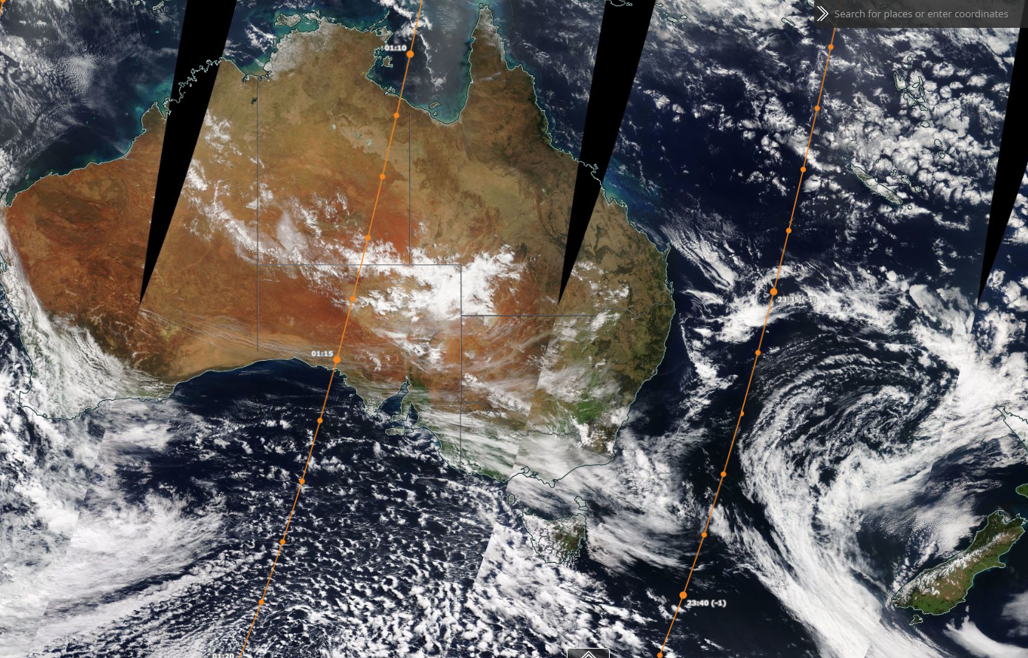
\includegraphics[width=\textwidth]{bilder/wrf/20T00_sat.png}
	\end{minipage}\hfill
	\begin{minipage}[c]{0.35\textwidth}
		 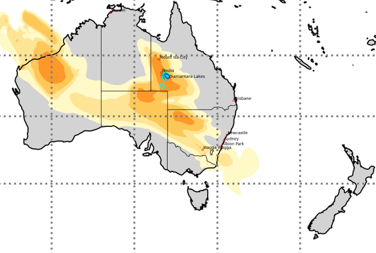
\includegraphics[width=\textwidth]{bilder/wrf/20T00_wrf.png}
	\end{minipage}\hfill
	\begin{minipage}[c]{0.29\textwidth}
		 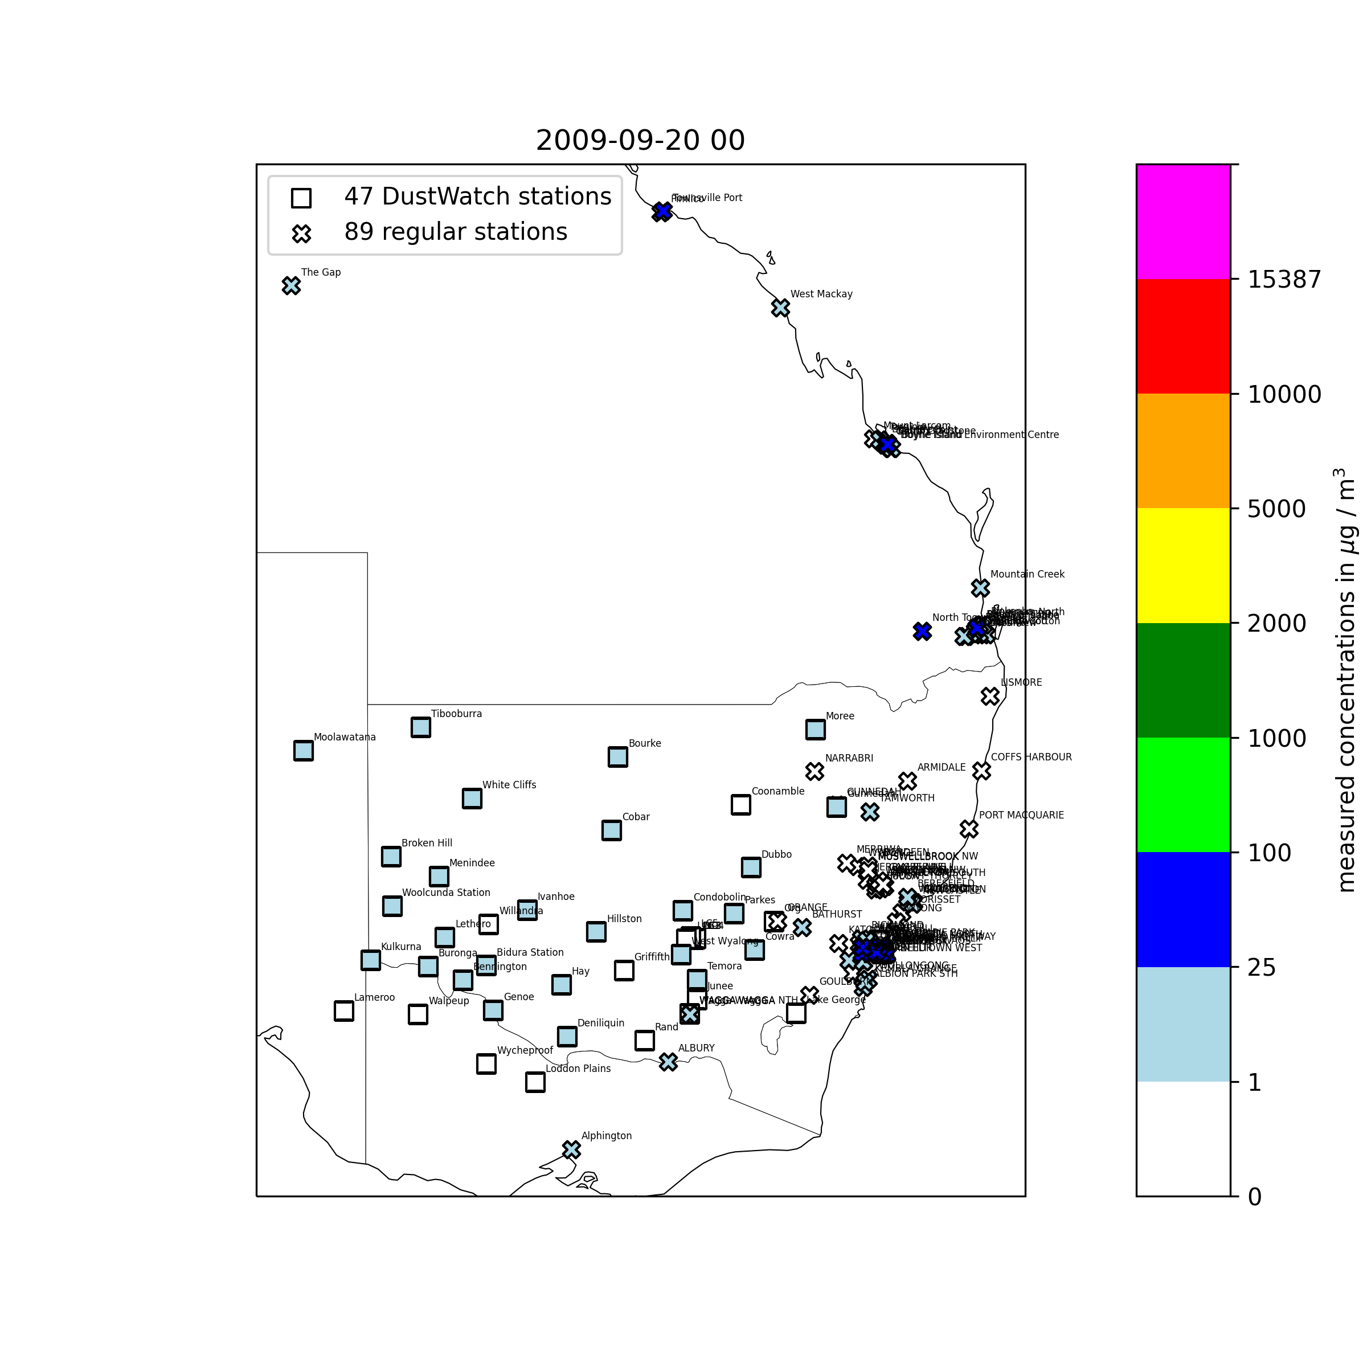
\includegraphics[width=\textwidth]{bilder/wrf/20T00_obs.png}
	\end{minipage}\hfill
	\begin{minipage}[c]{0.35\textwidth}
		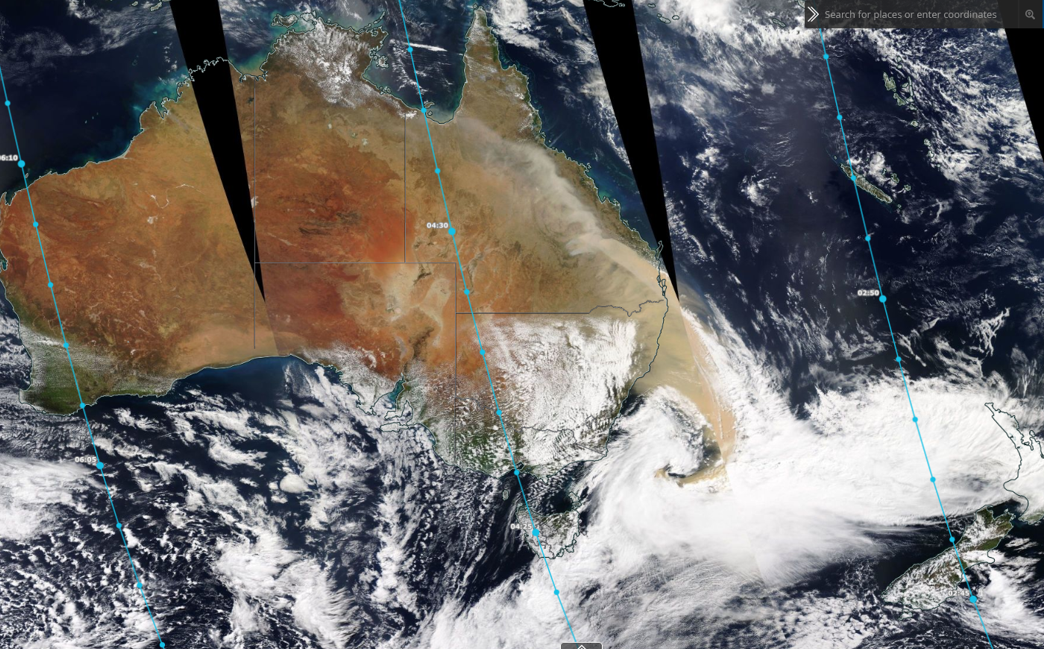
\includegraphics[width=\textwidth]{bilder/wrf/23T06_sat.png}
	\end{minipage}\hfill
	\begin{minipage}[c]{0.35\textwidth}
		 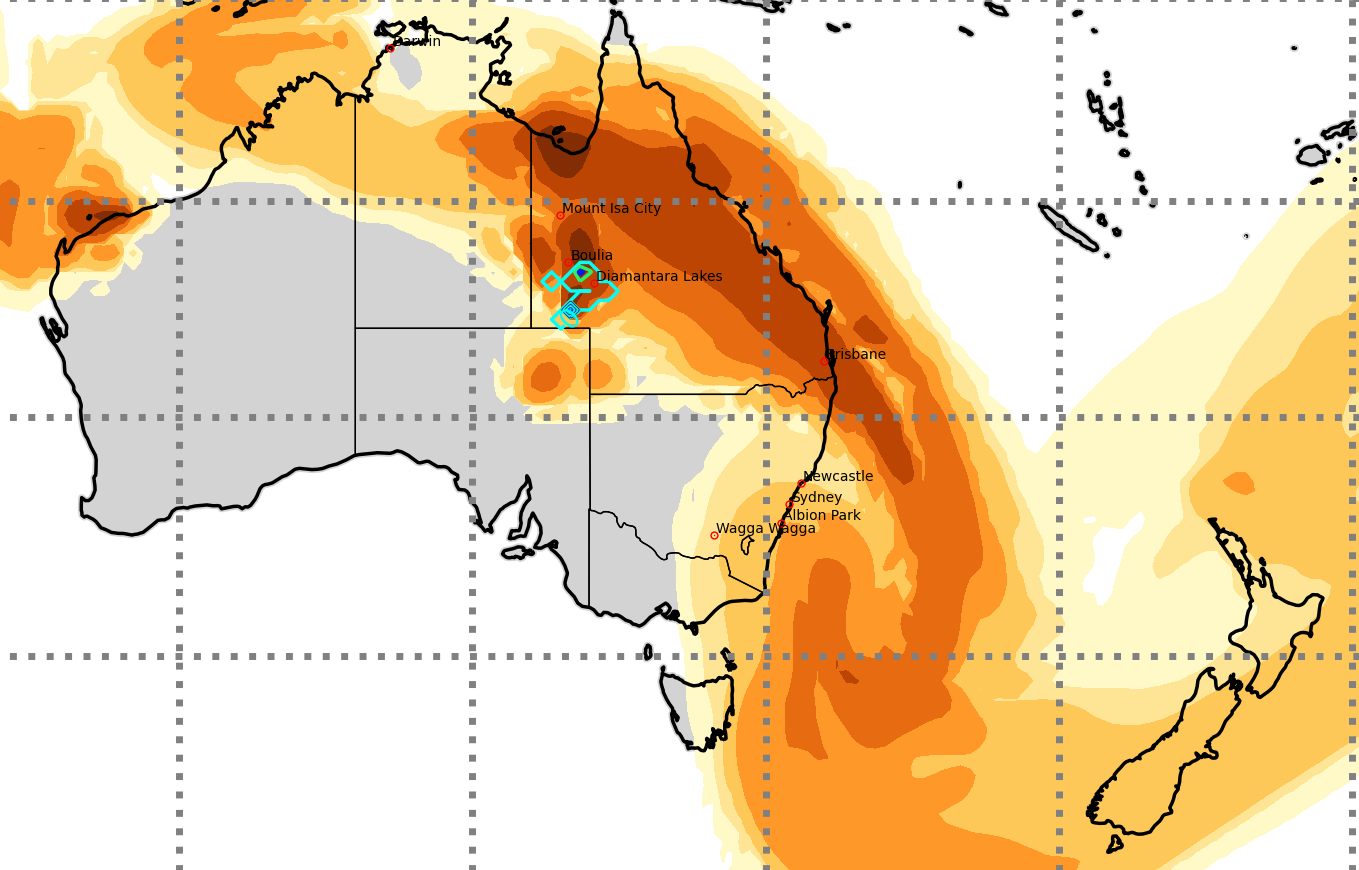
\includegraphics[width=\textwidth]{bilder/wrf/23T06_wrf.png}
	\end{minipage}\hfill
	\begin{minipage}[c]{0.29\textwidth}
		 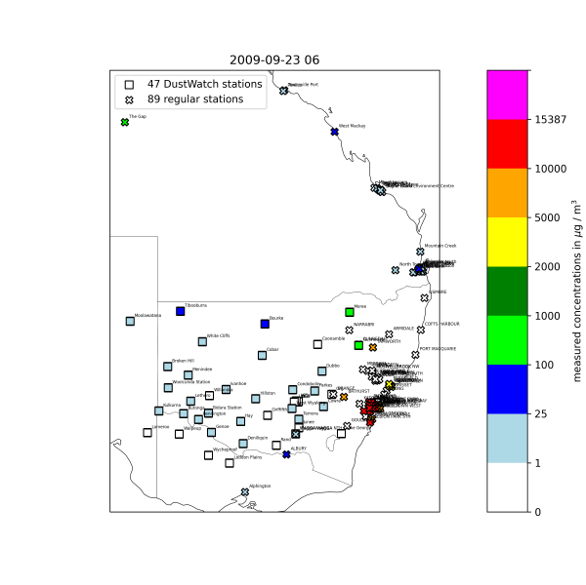
\includegraphics[width=\textwidth]{bilder/wrf/23T06_obs.png}
	\end{minipage}\hfill
	\begin{minipage}[c]{0.35\textwidth}
		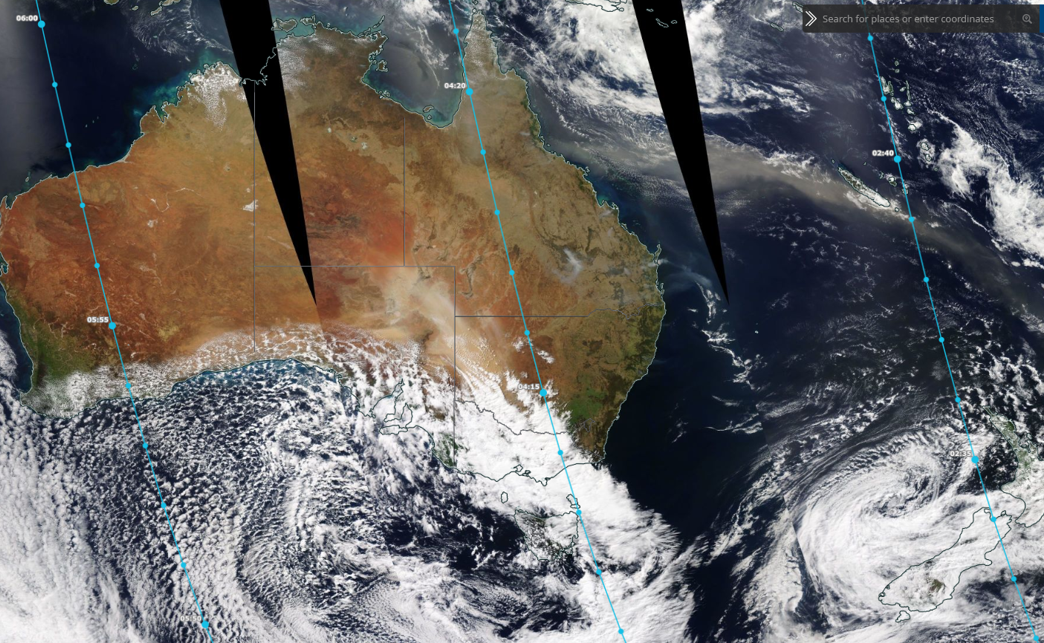
\includegraphics[width=\textwidth]{bilder/wrf/25T06_sat.png}
	\end{minipage}\hfill
	\begin{minipage}[c]{0.35\textwidth}
		 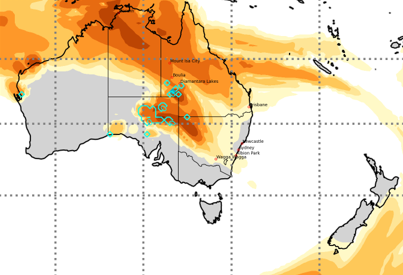
\includegraphics[width=\textwidth]{bilder/wrf/25T06_wrf.png}
	\end{minipage}\hfill
	\begin{minipage}[c]{0.29\textwidth}
		 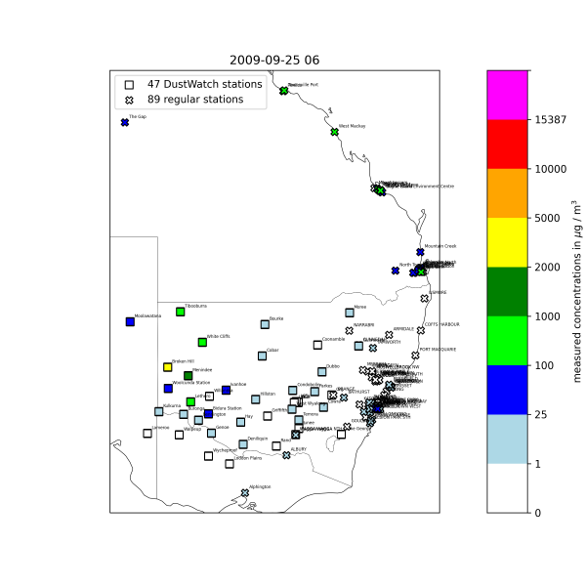
\includegraphics[width=\textwidth]{bilder/wrf/25T06_obs.png}
	\end{minipage}\hfill
	\begin{minipage}[c]{\textwidth}
		\captionsetup{format=hang, indention=0.0cm}
		\caption{Das muss ich irgendwie noch schöner machen....}
		\label{fig:wrf_sat}
	\end{minipage}
\end{figure}
Der Großteil des Staubs wird laut WRF-Modell aus der Region \textit{Channel Country} im Westen Queensland in der Nähe der \textit{Diamantina Lakes} emittiert. Diese Region wird grundsätzlich als Quelle für das Red-Dawn-Event vermutet (sh. Kapitel \textbf{XY}, \cite{Leys.2011}), allerdings bislang nicht als dominierende. Auf Abbildung \ref{fig:max_emis} wird deutlich, dass diese im Modell aber deutlich dominiert. Die Vermutung liegt nahe, dass ebendiese Emissionen zu den erhöhten (möglicherweise unrealistischen) modellierten Staubkonzentrationen im Nordwesten führen. Die Staubemissionen können im Modell aus verschiedenen Gründen überschätzt werden. Ein offensichtlicher Nachteil des im Modell implementierten Schemas zur Staubemission ist, dass nicht berücksichtigt wird, wie viel Staub am jeweiligen Gitterpunkt maximal emittiert werden kann. Ist eine Region also einmal als Staubquelle mit einer entsprechenden Größenordnung definiert, kann bei entsprechenden Windstärken theoretisch beliebig viel Staub emittiert werden. Dies soll in späteren Versionen durch eine \textit{Budgetierung} des maximal \textit{emissionsfähigen} Staubs an der Oberfläche implementiert werden, sodass die Emission stoppt, nachdem das Budget aufgebraucht ist. Durch neue Ablagerungen von Staub (Deposition) kann das Budget dann wieder aufgefüllt werden. Anschließend wären die Emissionen \textit{zeitlich} limitiert.
\begin{figure}
\centering
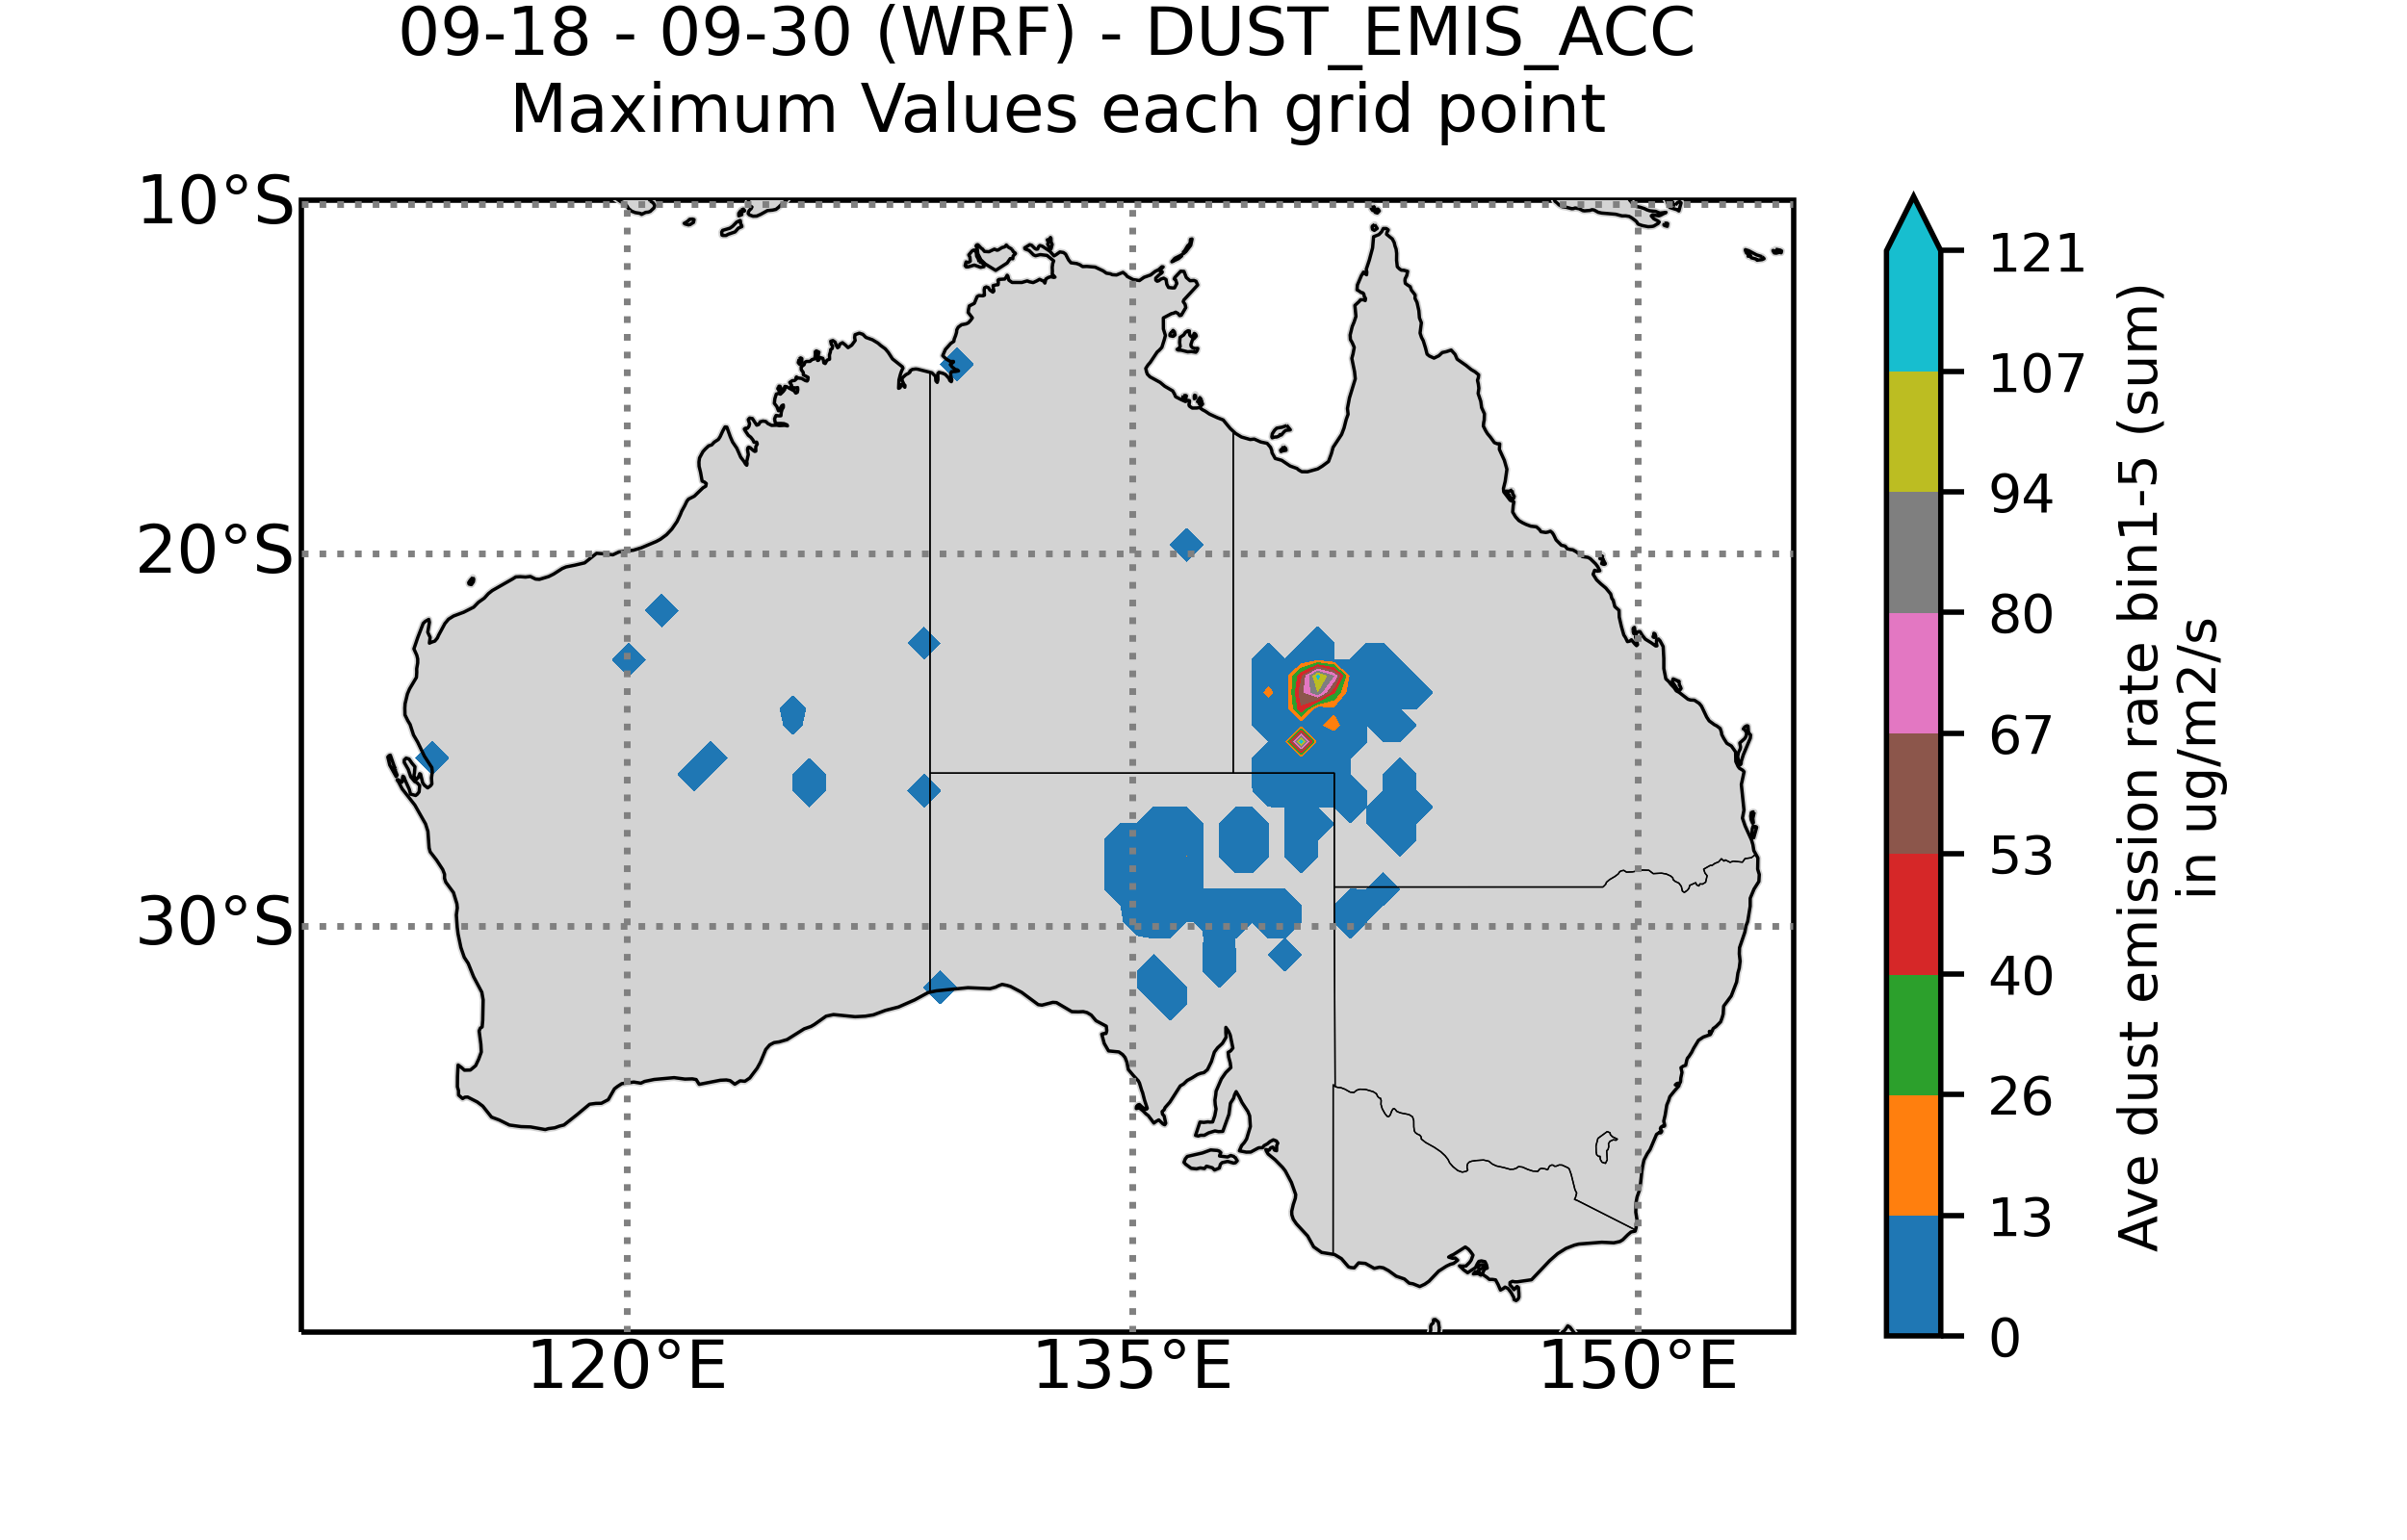
\includegraphics[width=\textwidth]{bilder/wrf/max_emis.png}
\caption{Darstellung der maximalen Staubemissionen über alle Zeiten je Gitterpunkt. Die Variablen DUST_EMIS_ACC1..5 beschreiben die über den letzten Zeitschritt (hier 3 Stunden) gemittelten Werte der Staubemissionen und wurden hier aufsummiert.} \label{fig:max_emis}
\end{figure}
Neben der zeitlichen Beschränkung beeinflussen verschiedene Parameter die zeitunabhängige Größenordnung der Emissionen. Insbesondere entscheidend für das Emissionspotential ist die Rauheit des Geländes. Dies stellt in Simulationen stets ein Problem dar, da die räumliche Auflösung eines diskreten Modells nie alle beliebig kleinen Elemente abdecken kann. Stattdessen wird jedem Gitterpunkt ein Parameter zugeordnet, der die Rauheit repräsentiert und die Emissionen stellvertretend regulieren soll. Im vorliegenden WRF-Modell werden dazu die Vegetationsparameter angepasst \textbf{LAI oder VEGFRA?}, da Vegetation einen vergleichbaren Einfluss nimmt wie Rauheit, bzw. ebenfalls eine gewisse Rauheit darstellt. Diese Informationen, welche Größe die Parameter an welchem Gitterpunkt annehmen, werden durch Geogrid-Daten in das WRF-Modell gegeben. In Abbildung \label{fig:emis_ctrl} sind einige der relevanten Parameter dargestellt. Es wird deutlich, dass die Zelle mit den höchsten Emissionen (\textit{1}) im Vergleich zu den Nachbarzellen etwas andere Werte erreicht, was zu verstärkten Emissionen führt. Da angenommen wird, dass die sehr hohen Emissionen unrealistisch sind, wurde der Blattflächenindex (LAI) an den 10 Gitterpunkten mit den höchsten Emissionen gezielt korrigiert. Dies führt zu einer veränderten Rauheit und soll die Emissionen auf ein adäquates Level limitieren.

\begin{figure}
\centering
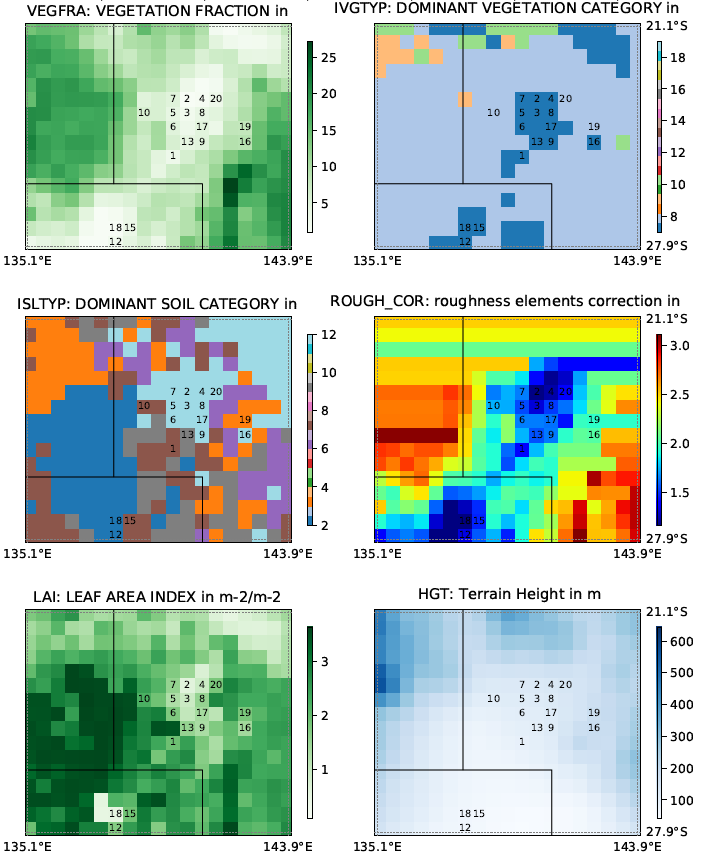
\includegraphics[width=0.7\textwidth]{bilder/wrf/emis_ctrl.png}
\caption{Absolute Werte einiger konstanter Parameter im WRF-Modell für die Region mit hohen Emissionen, die die Staubemissionen regulieren können. Die Zahlenwerte 1 bis 20 geben die Rangordnung der Staubemissionen an. Das heißt, Gitterpunkt 1 erreicht die höchste Emission, 2 die zweithöchste usw.}

\end{figure}



\subsection{Staubkonzentrationen}
- Hohe Konzentrationen an der Oberfläche werden durch Modell ungenügend beschrieben (siehe DUST_ACC_ auf zlevel 0 (geländefolgend)). DUSTLOAD über ganze Atmosphärensäule allerdings schon eher. Sehr sehr hohe Konzentrationen  ($>$ 10kg pro qm) später im Norden.
\section{Staubquellen und Emissionen}
Staubquellen gemäß \citep{Leys.2011}
\begin{enumerate}
\item lower Lake Eyre Basin
\item grazing lands of north western NSW
\item mining areas around Cobar und Broken Hill
\item Channel Country of western Queensland
\end{enumerate}
Laut Modell enorm hohe Emissionen zwischen Diamantara Lakes und Boulia (western Queensland). Laut \citet{Deckker.2014} konnte Lake Torrins als Quelle für Staub der bei Canberra gefallen ist identifiziert werden. Diese Region ebenfalls Bestandteil des Modells. Die \textit{Fingerabdruckanalyse} von \citet{Deckker.2014} ist leider dadurch beschränkt, dass nur Proben aus den beiden (im Vergleich zur Ausdehnung der Staubwolke) sehr südlich gelegenen Städten Canberra und Eden verwendet werden konnten. Die damit abgeleiteten Staubquellen sind also vermutlich für den Großteil des Ereignisses nicht repräsentativ. -  Benutzt man die Unterteilung in \citet{OLoingsigh.2017}, dann laut Modell Region (2) Channel Country mit Abstand größte Quelle, aber auch (3) Lake Eyre (A) and South Simpson desert ephemeral lakes region, (4) South Strzelecki desert and Lake Frome (B) subbasin, (5) Lakes Torrens (C). -  Staub beschreibt eine bestimmte Signatur, die von den Eigenschaften des Sediments unterschieden werden kann, in welchem sich der Staub abgelagert hat. Die besondere Signatur kann nach \citet{Marx.2018} durch verschiedene Mechanismen verursacht werden:
\begin{enumerate}
\item Transport
\item geochemisch oder mineralogisch
\item \textit{Fingerabdruck} der Herkunftsregion
\item anthropogene Effekte
\end{enumerate}
\section{Zusammenfassung und Ausblick}
\newpage
\printbibliography
\appendix
\section{Anhang}
\subsubsection{Maximum Kovarianz Analyse} \label{sec:mca}
Durch die hohe Abhängigkeit von der chemischen Zusammensetzung und den Strömungsverhältnissen sind die Chlorophyll-a-Konzentrationen sehr heterogen verteilt. In Abbildung \ref{fig:chla} wird das turbulente Muster beispielhaft deutlich. Insbesondere die Vergleichbarkeit mit den Perzentilen (sh. Kapitel \ref{sec:timeseries}) ist dadurch vom eingrenzten Gebiet abhängig und somit eingeschränkt. Es wird angenommen, dass (besonders im tasmanischen Meer) ein Großteil der Gitterzellen innerhalb der Klimadaten sowohl Jahre mit hohen als auch solche mit niedrigen Konzentrationen repräsentiert hat, wohingegen \textit{benachbarte} Zellen, die bspw. einer anderen Strömungslinie folgen, völlig unterschiedliche Werte aufweisen können. \\
Es soll der Zusammenhang zweier diskreter Variablen $E$ (Eiseneintrag) und $P$ (Chlorophyll-a-Konzentrationen untersucht werden). Voraussetzung für die Maximum Kovarianz Analyse ist, dass für beide gleich viele $N_t$ Zeitschritte vorliegen. Die Anzahlen der Gitterpunkte $N_E$ bzw. $N_P$ können voneinander abweichen. Der Zusammenhang der Variablen wird bei dieser statistischen Methode unabhängig von deren räumlicher Lokation untersucht. Das heißt, es ist auch ein Einfluss von weit voneinander entfernten Gitterpunkten aufeinander möglich. Dies ist bei den Staubdepositionen nicht unbedingt zu erwarten, da eine Reaktion des Phytoplanktons vermutlich in naher Umgebung zum Staubeintrag passiert. Allerdings \textit{befreit} diese Unabhängigkeit gleichzeitig von der Anforderung, für beide Variablen dieselben Koordinaten bzw. räumlichen Auflösungen zu verwenden und/oder etwaigen Transport durch die Oberflächenströmungen zu berücksichtigen. Werden die beiden räumlichen Dimensionen (Nord-Süd und Ost-West) auf nur eine räumliche Dimension (hier mit dem  Index $k$) reduziert, dann lassen sich die kompletten  Zeitreihen aller Gitterpunkte gleichzeitig in Form von Matrizen darstellen. Im folgenden meinen hoch gestellte Indizes die \textit{Spalte} und die unteren Indizes die \textit{Zeile} der jeweiligen Matrix. Die Matrizen in \ref{eq:E_and_P} enthalten $N_t$ Zeitschritte in den Zeilen und $N_E$ bzw. $N_P$ Gitterpunkte in den Spalten.
\begin{equation}
\textbf{E} = \begin{pmatrix} E_{1}^1 & .. & E_{N_E}^1 \\ .. & .. & .. \\ E_{1}^{N_t} & .. & E_{N_E}^{N_t} \\ \end{pmatrix} \text{ und } \textbf{P} = \begin{pmatrix} P_{1}^1 & .. & P_{N_P}^1 \\ .. & .. & .. \\ P_{1}^{N_t} & .. & P_{N_P}^{N_t} \\ \end{pmatrix} \label{eq:E_and_P}
\end{equation}
Da im Rahmen der Kovarianzanalyse \textit{Abweichungen}, also Varianzen von einem \textit{normalen} Zustand untersucht werden, wird jeder Eintrag $P_k^t$ (analog für $E_k^t$) normalerweise noch durch Subtraktion des zeitlichen Gitterpunkt-Mittelwertes für jede Zeitreihe als Anomalie von ebendiesem Mittelwert berechnet:
\begin{equation}
P_{a,k}^t = P_k^t - \frac{1}{N_t} \sum\limits_{n=1}^{N_t} P_k^n = P_k^t - \overline{P_k}
\end{equation}
Um einen möglichen Trend (sh. Kapitel \ref{sec:timeseries}) zu eliminieren, soll bei den Chlorophyll-a-Konzentrationen anstatt des Zeitserien-Mittelwertes allerdings der klimatische Mittelwert verwendet werden, sh. Gleichung \ref{eq:cli_anomalie}. Für die Eisendepositionen wird angenommen, dass der klimatische Mittelwert annähernd 0 beträgt, sodass alle Einträge als positive Anomalie betrachtet wird. Es erfolgt demnach keine Subtraktion. Allerdings wird das Gebiet räumlich auf den Ozean beschränkt, sodass Einträge auf Landflächen keinen Einfluss nehmen. Darüber hinaus können wie in Kapitel \ref{sec:timeseries} sowohl die Gitterpunkte von $\textbf{E}$ als auch von $\textbf{P}$ auf Regionen beschränkt werden, in denen die Eisendepositionen eine bestimmte Schwelle überschreiten. Anschließend werden alle Werte mithilfe der Standardabweichung $\sigma$ normiert, damit einige wenige Gitterpunkte mit sehr hohen Werten/Varianzen später keinen überproportionalen Einfluss auf das Gesamtergebnis nehmen:
\begin{equation}
\hat{E}_k^t =  \frac{1}{\sigma} \cdot E_k^t \text{ für } k = 1,..,N_E 
\end{equation}
mit der Varianz
\begin{equation}
\sigma^2 = \frac{1}{N_t} \sum\limits_{n=1}^{N_t-1}(E_k^n-\overline{E_k})^2
\end{equation}
Nach diesen Vorarbeiten (Normierung analog für \textbf{P}$_a$) wird die Kovarianzmatrix \textbf{X}$\in \mathbb{R}^{N_E \times N_P}$ berechnet ($\textbf{\^{E}}^T$ meint die transponierte Matrix):
\begin{equation}
\textbf{X} = \frac{1}{N_t} \cdot \textbf{\^{E}}^T \cdot \hat{\textbf{P}}_a
\end{equation}
Diese enthält alle Informationen über die zeitlichen Kovarianzen aller möglichen Kombinationen eines jeden Gitterpunktes der einen Variable mit jedem Gitterpunkt der anderen Variable. Mithilfe der Singulärwertzerlegung lassen sich diese Informationen in Hauptkomponenten zerlegen.
\begin{equation}
\textbf{X} = \textbf{U} \cdot \textbf{S} \cdot \textbf{V}^T
\end{equation}
hierbei ist \textbf{S}$\in \mathbb{R}^{N_E \times N_P}$ eine Diagonalmatrix und enthält die $\min(N_E,N_P)$ Singulärwerte $S_k$ in dem Betrag nach \textit{absteigender} Reihenfolge. Dementsprechend enthalten i.d.R. die ersten Singulärwerte einen überproportional großen Informationsgehalt gegenüber den letzten, die möglicherweise (abhängig von den Anforderungen an die Genauigkeit) vernachlässigt werden können. Die Spalten der orthogonalen Matrizen \textbf{U}$\in \mathbb{R}^{N_E \times N_E}$ und \textbf{V}$\in \mathbb{R}^{N_P \times N_P}$ sind die linken, respektive rechten Singulärvektoren zur Kovarianzmatrix \textbf{X}. 
\begin{equation}
\hat{S_m}= \frac{1}{\sqrt{S_m\cdot N_t}}\textbf{ für } m=1,..,\min(N_E,N_P)
\end{equation}
Durch Matrixmultiplikation der ursprünglichen Matrizen mit den Singulärvektoren und -werten werden Zeitreihen der sogenannten \textit{Principal Components} erzeugt, welche in Form der Matrizen \textbf{PC}$_E\in \mathbb{R}^{N_t \times N_E}$ und \textbf{PC}$_P\in \mathbb{R}^{N_t \times N_P}$ gespeichert sind. Die jeweils $k$-te Spalte enthält die zum $k$-ten Singulärwert zugehörige Zeitreihe.
\begin{align}
\textbf{PC}_E &= \hat{\textbf{E}} \cdot \textbf{U} \cdot \hat{\textbf{S}}^T \\ \textbf{PC}_P &= \hat{\textbf{P}}_a \cdot \textbf{V} \cdot \hat{\textbf{S}}
\end{align}
Die Singulärvektoren selbst beschreiben das räumliche Muster zum zugehörigen Singulärwert und werden auch \textit{EOF} (Empirical Orthogonal Functions) genannt. Die so darstellbaren zeitlichen (PC's) und räumlichen (EOF) Strukturen werden auch als jeweiliger \textit{Modus} bezeichnet ($m$-ter Singulärwert und -vektor beschreiben $m$-ten Modus). Zur späteren übersichtlichen Darstellung in Kapitel \ref{sec:auswertung} werden die PC's und EOF's durch die Maximalwerte noch auf 1 normiert:
\begin{align}
\widehat{\text{PC}}_{E,m}^t &= \frac{\text{PC}_{E,m}^t}{\max\limits_n(|\text{PC}_{E,m}^n|)} \text{ für } m = 1,..,\min(N_E,N_P), t = 1,..,N_t \\
\widehat{\text{PC}}_{P,m}^t &= \frac{\text{PC}_{P,m}^t}{\max\limits_n(|\text{PC}_{P,m}^n|)} \text{ für } m = 1,..,\min(N_E,N_P), t = 1,..,N_t
\end{align}
\begin{align}
\widehat{\text{EOF}}_{E,k}^m &= \frac{\text{U}_{k}^m}{\max\limits_n(|\text{U}_{n}^m|)} \text{ für } m = 1,..,\min(N_E,N_P), k = 1,..,N_E \\
\widehat{\text{EOF}}_{P,k}^m &= \frac{\text{V}_{k}^m}{\max\limits_n(|\text{V}_{n}^m|)} \text{ für } m = 1,..,\min(N_E,N_P), k = 1,..,N_P 
\end{align}

\section{Gabric.2016}

\begin{itemize}
\item Tasman Sea $25^\circ$ S bis $40^\circ$ S Untersuchungsareal
\item data: Chl + aeorosol optical depth (AOD)
\begin{itemize}
\item chl data: daily + 8 day MODIS-AQUA
\item AOD data: 550 nm, 4km resolution
\end{itemize}
\item divided into $5^\circ$ lattitude band
\item DVR kumulativ
\item Hovmoller Plots (x: zeit, y: latidude, longitude)
\item cloud processing / wet deposition wichtig
\item Response hauptsächlich südlich der tasmanischen Front ($\approx 32^\circ$ S)
\item Staubdeposition weiter im Norden
\end{itemize}

\end{document}
